\documentclass[cclicense]{hmcthesis}

\usepackage{util}
\usepackage{math}

\usepackage{extarrows}
\usepackage{kbordermatrix}

\usepackage{makeidx}
\makeindex

\newcommand*{\x}[1]{\ensuremath{X^{(#1)}}}
\providecommand*{\xs}{\mathcal X}
\providecommand*{\ms}{\mathcal M}
\providecommand*{\ns}{\mathcal N}
\providecommand*{\N}{\mathbb{N}}
\newcommand*{\vbar}{\;\big\vert\;}
\DeclareMathOperator*{\argmax}{arg\ max}

\newcommand*{\mle}{\mathrm{mle}}
\newcommand*{\emp}{\mathrm{emp}}

\numberwithin{equation}{chapter}
\numberwithin{thmcounter}{chapter}

\title{Log-Linear Models on Homogeneous Spaces}
\author{Aaron Pribadi}
\thesisyear{2012}
\advisor{Michael Orrison}
\reader{Weiqing Gu}

\begin{document}

\frontmatter

\maketitle

\tableofcontents




\chapter{Abstract}
    This will be an abstract.

\chapter{Acknowledgements}
    There will be acknowledgements.

\mainmatter

\chapter{Discrete Models and Linear Spaces}

    \section{Discrete Data}

    Throughout, we are primarily concerned with the analysis of discrete data,
    for which each observation has only finitely many possible outcomes.

    One fundamental assumption is that repeated observations are independent and
    identically distributed random variables.  That is, the observations $\x 1,
    \ldots, \x m$ are random variables, and each is distributed according to the
    same underlying probability distribution, $\x i \sim p$.  Given an observed
    set of values for the $\x i$, a basic objective is to estimate the
    underlying probability distribution $p$.

    Let each $\x i$ take a value from the sample space $\xs$.  Throughout, we
    assume that $\xs$ is a finite set.  Because the order of the observations
    does not matter, we can summarize the observations with the counts
    \begin{equation*}
        u(x) = \pdel{\text{the number of $i$ for which $\x i = x$}}
    \end{equation*}
    for $x \in \xs$.  If the number of states $|\xs|$ is small relative to the
    number of samples $m$, then the empirical distribution
    \begin{equation}
        p_\emp(x) = \frac{u(x)}{m}
        \label{eq:empirical}
    \end{equation}
    is a useful estimate of the true distribution $\x i \sim p$.

    It is sometimes the case that $|\xs|$ is very large.  Without a
    correspondingly large number of samples, the empirical distribution $p_\emp$
    may not adequately capture the underlying distribution $p$.  Such sample
    spaces arise naturally in a variety of situations.  The sample space for
    discrete multivariate data, which consists of observations with multiple
    components, is a cartesian product $\xs = \xs_1 \times \cdots \times \xs_k$
    of several finite sets.  Each component space $\xs_i$ can correspond to the
    assignment of some label to each observation.  For example, a person can
    have an eye color, a hair color, a handedness, a gender, etc.  If each
    variate has approximately the same number of possible values, then the
    number of states is exponential in the number of variates.  Another example
    of a large sample space is the space of rankings of $n$ items.  This could
    occur if voters were asked to rank candidates in an election.  If all $n$
    items are ranked, then the sample space has $n!$ possible outcomes.  For the
    empirical distribution to produce a good estimate of the underlying
    distribution, a prohibitively large number of samples is required.

    In order to analyze data with a large number of states, it is often fruitful
    to restrict which distributions we consider.  In each of the examples from
    above, the sample space has some combinatorial structure.  Our goal is to
    use the structure of the underlying space of states in order to better
    analyze data.

    \begin{example}
        The UCI database \citep{UCIData} contains a large number of data sets
        used for the evaluation of machine learning techniques.  The
        Congressional Voting Records data set contains Congressional voting
        records on a number of key issues.
        \begin{figure}[H]
            \centering
            \begin{verbatim}
            1) democrat   n y y n y y n n n n n n y y y y
            2) republican n y n y y y n n n n n y y y n y
            3) democrat   y y y n n n y y y n y n n n y y
            4) democrat   y y y n n n y y y n n n n n y y
            5) democrat   y n y n n n y y y y n n n n y y
            \end{verbatim}
            \vspace{-1.5\baselineskip}
            \caption{A few points from the Congressional Voting Records
            data set.}
        \end{figure}
        \noindent Ignoring missing values, e.g. where representatives did not
        vote, each variate has two possible values, either $\{\texttt{democrat},
        \texttt{republican}\}$ or $\{\texttt{yes}, \texttt{no}\}$.  Thus, the
        sample space may be written as $\xs = \{0, 1\}^7$, the set binary
        strings with 7 bits.  As $|\xs| = 2^{17} = 131072$ is a large number,
        some assumptions about potential distributions are needed to make sense
        of the data.
        \label{ex:voting}
    \end{example}


    \section{The Simplex and Statistical Models}

    We take a geometric view of statistical models.  This perspective allows
    statistical problems to be attacked with a large range of useful tools.

    A probability distribution on a finite set $\xs$ can be thought of as a
    real-valued function $p \in L(\xs)$ subject to the restrictions that
    $\sum_{x\in \xs} p(x) = 1$ and that $p(x) \ge 0$ for all $x \in \xs$.  The
    function $p$ is the probability mass function.  Finite sets are particularly
    convenient because we can always work with a probability mass function, and
    because the probability mass function is always embedded in an ambient
    finite dimensional vector space.  The space of all distributions on $\xs$ is
    a geometric object.
    
    \begin{definition} 
        \index{simplex}
        The \emph{standard simplex} of dimension $N$ is the subset
        \[
            \Delta_N = 
            \left\{(p_1, \ldots, p_{N+1}) \in \R^{N+1} \vbar 
            \sum_{i=1}^{N+1} p_i= 1, p_i \ge 0 \right\} 
        \]
        of $\R^{N+1}$.  If the appropriate dimension is either clear in context
        or irrelevant, then we may write $\Delta$, omitting the subscript.
    \end{definition}

    The simplex is a generalization of an equilateral triangle.  Low-dimensional
    simplices are familiar shapes; $\Delta_0$ is a point, $\Delta_1$ is a line
    segment, $\Delta_2$ is a triangle, and $\Delta_3$ is a tetrahedron.
    \begin{figure}[H]
        \centering
        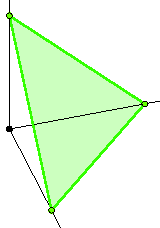
\includegraphics[scale=1]{2-simplex.pdf}
        \caption{The 2-simplex.}
    \end{figure}
    There is a one-to-one correspondence between probability distributions on
    the set $\xs = \{x_1, \ldots, x_{N+1}\}$ and points in the simplex
    $\Delta_N$; the probability $p(i)$ is equal to the value of the coordinate
    $p_i$.  We therefore identify the two concepts with each other.
    Because the space of all probability distributions is a geometric
    object, it is easy to talk about specific families of probability
    distributions.
    \begin{definition}
    A \emph{statistical model} is a subset $\ms \subset \Delta$ of the
    probability simplex.  A \emph{parametrized model} $\ms$ with parameter space
    $\Theta$ is specified by a surjective map $\Theta \to \ms$.  We usually
    write $p_\theta$, with $\theta \in \Theta$, to denote a distribution from a
    parametrized model.
    \end{definition}
    Many statistical models have been studied and employed for the analysis of
    data, and the selection of an appropriate model is a delicate question.  In
    Section~\ref{sec:linear-models} we introduce a family of models with
    convenient properties.

    In an ideal situation, there is a hypothesis for an underlying mechanism
    producing observable results.  In that case, a particular choice of model is
    easy to justify.

    \begin{example}[Binomial model]
    The distribution $\mathrm{Binom}(N, \alpha)$ models the number of heads
    produced by $N$ independent `coin tosses', where $0 \le \alpha \le 1$ is
    the probability that a single toss produces a head.  It is defined
    \[
        p_\alpha(k) = {N \choose k} \alpha^k(1-\alpha)^{n-k}.
    \]
    for $k \in \{0, \ldots, N\}$.  The map $\alpha \mapsto p_\alpha$
    determines a parametrized statistical model.  The statistical model is a
    curve, i.e. a one-dimensional subset, of the simplex.  

    The model $\mathrm{Binom}(2, \alpha)$ simulates two coin flips.  The three
    coordinates of a point in the model measure the probabilities that zero,
    one, and two heads will occur, respectively.
    \begin{figure}[H]
        \centering
        \vspace*{-0.2cm}
        \scalebox{1}{ 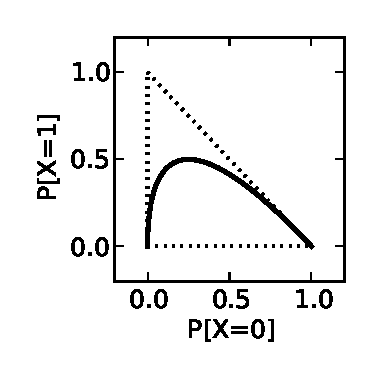
\includegraphics[scale=0.7]{images/binomial.pdf} }
        \vspace*{-0.5cm}
        \caption{The binomial model for $N=2$. Make this 3-D?}
        \label{fig:binomial}
    \end{figure}
    \noindent As the parameter $\alpha$ varies over $[0,1]$, the statistical
    model traces out the curve 
    \[
        \alpha \longmapsto \big((1-\alpha)^2, 2\alpha(1-\alpha), \alpha^2\big)
    \]
    in the simplex $\Delta_2$ (see Figure~\ref{fig:binomial}).  

    If we knew that a coin was being flipped twice, and did not know the odds of
    the coin, then the model $\alpha \mapsto \mathrm{Binom}(N, \alpha)$ would be
    an appropriate choice for analysis.
    \end{example}

    \begin{example}[Independence]
        The independence model on a sample space $\xs = \xs_1 \times \cdots
        \times \xs_k$ assumes that each variate is independent.  For a
        distribution $p$ on $\xs$, the variates are said to be independent if
        $p$ factors as
        \[
            p(x) = p_1(x) \cdots p_k(x)
            \qquad
            \text{where}
            \qquad
            p_i(x) = \sum_{\stackrel{y \in \xs}{x_i = y_i}} p(y)
        \]
        for all $x = (x_1, \ldots, x_k) \in \xs$.  Each factor $p_i(x)$ is a
        function only of the $i$th component $x_i$.  Despite this simplistic
        assumption, the independence model is surprisingly effective in many
        situations, e.g. for naive Bayes classifiers.  
        
        The map 
        \begin{align*}
        \Delta_{|\xs_1|-1} \times \cdots \Delta_{|\xs_k|-1} 
        &\to \Delta_{|\xs| - 1} \\
        (p_1, \ldots, p_k) &\mapsto p_1 \cdots p_k
        \end{align*}
        gives a parametrization of the independence model.  Counting dimensions
        indicates that the independence model imposes strict limitations on
        potential distributions.  The parameter space has dimension
        \[
            \dim 
            (\Delta_{|\xs_1|-1} \times \cdots \Delta_{|\xs_k|-1})
            =
            |\xs_1| + \cdots + |\xs_k| - k
        \]
        whereas the space of all distributions on $\xs$ has dimension 
        \[
            \dim(\Delta_{|\xs| - 1})
            =
            |\xs_1| \cdots |\xs_k| - 1.
        \]
        If the variates are binary, as in Example~\ref{ex:voting}, then the
        model has dimension $k$ and the whole simplex has dimension $2^k - 1$.
        
        The independence model is employed in part because it is easy to
        interpret.  In effect it states that the variates do not affect each
        other.
        \label{ex:independence1}
    \end{example}
    
\section{Likelihood and Model Complexity}
    In the analysis of data, there is a tension between how well an explanation
    fits the observed data, and how well such an explanation can be expected to
    generalize to new data.  While we do not explore all nuances of this topic,
    we do introduce a few fundamental concepts.

    One way to measure how well a distribution matches data is to ask the
    question, ``How likely is the data, given the distribution?''  A maximum
    likelihood estimate quantifies whether a model contains distributions that
    match well.

    Let $\ms = \{p_\theta : \theta \in \Theta\}$ be a parametrized statistical
    model.  Suppose that some data $Z = \{z_1, \ldots, z_m\}$ are observed.  It
    is generally assumed that the data has been drawn from independent and
    identically distributed samples following an unknown true distribution from
    the model.from the model.
    
    \begin{definition}
    The \emph{likelihood function} of $\theta \in \Theta$ given the data $Z$ is
    \[
        L(\theta; Z) = \prod_{i=1}^n p_\theta(z_i).
    \]
    It is the probability that the observed data $Z$ would occur if the samples
    followed $p_\theta$.  Oftentimes, the \emph{negative log-likelihood}
    \[
        -l(\theta; Z) = -\log L(\theta; Z) = -\sum_{i=1}^n \log p_\theta(z_i).
    \]
    is used in lieu of the likelihood.  The negative log-likelihood is useful
    because the contributions to $l(\theta; Z)$ from the observations $z_i$ are
    additive and each acts as a `penalty' or `loss'.
    \end{definition}
    \begin{definition}
    The \emph{maximum likelihood estimate} of the true parameter is the
    parameter 
    \[
        \theta_\mle = \argmax_{\theta \in \Theta} L(\theta; Z)
    \]
    that maximizes the likelihood of the data, or that equivalently minimizes
    the negative log-likelihood of the data.  In some cases, we identify the
    parameter $\theta$ with the distribution $p_\theta$ and use the term
    `maximum likelihood estimate' to refer to the distribution $p_\mle$ from the
    model that maximizes the likelihood.
    \end{definition}

    \begin{note}
        The fact that a maximum likelihood estimate might not exist is tacitly
        ignored.  Indeed $\{L(\theta; Z) \mid \theta \in \Theta\}$ might be an
        open set, and the map $\theta \mapsto L(\theta; Z)$ might not be
        surjective.  In applications with real data, it is often the case that a
        precise maximum likelihood estimate is not necessary, and that an
        approximate value is sufficient.
    \end{note}

    The distribution $p_\mle$ from the maximum likelihood estimate is the best
    one possible from the model.  Notice that is $\ms \subset \ns$ are two
    statistical models, then the maximal likelihood from $\ms$ is less than or
    equal to that from $\ns$.  Thus `size' of the model determines how good of a
    distribution is possible.
    \begin{example}
        Suppose that the model does not restrict distributions at all, i.e.
        that the model is the whole simplex.  Then the maximum likelihood
        estimate is the empirical distribution $p_\emp(x) = u(x) / \sum_{y \in
        \xs} u(y)$ as in \eqref{eq:empirical}.
    \end{example}
    \begin{example}[Independence]
        Recall the independence model from Example~\ref{ex:independence1}.  The
        maximum likelihood estimate for the independence model is
        \[
            p_\mle(x) = \frac{u_1(x_1)}{m} \times \cdots \times \frac{u_k(x_k)}{m}
        \]
        where $x = (x_1, \ldots, x_k)$, $m$ is the number of samples, and
        $u_i(x_i)$ is the number of times that the $i$th variate of the
        observation is $x_i$.  In other words, we get a maximum likelihood
        estimate of each variate separately with its empirical distribution, and
        take the product distribution.
    \end{example}

    A larger model is deemed to contain more `complex' distributions.  The
    trade-off is that a larger model allows for probability distributions that
    fit the observed data better, but that might not generalize as well to
    subsequent observations.  This trade-off between model complexity and
    predictive power can be approached in a number of ways, and is explored in
    standard literature.  Chapter 7 of \citep{EOSL} is one reference.  
    
    There are at least two common methods to limit model complexity.
    \begin{itemize}
    \item We can require that the estimated distribution $p$ is contained within
    some model $\ms \subset \Delta$.
    \item We can minimize $-l(p) + \pi(p)$, the negative log-likelihood with an
    additional penalty term measuring the complexity of $p$.
    \end{itemize}
    Two criteria with complexity penalties are the Akaike information criterion
    and the Bayesian information criterion, defined
    \begin{align*}
        \mathrm{AIC} &= 2\pdel*{-l(p) + d} \\
        \mathrm{BIC} &= 2\pdel*{-l(p) + \frac{d \log(m)}{2}}
    \end{align*}
    where $d$ is the dimension of the parameter space $\Theta$ and $m$ is the
    number of samples.  These have different motivations, which are described in
    the above reference.

\section{Linear and Log-Linear Models}
    \label{sec:linear-models}
    
    The selection of distributions can be treated as a problem in function
    estimation.  From the data we construct the empirical distribution \mbox{$p_\emp
    \in L(X)$}, and we wish to find another function $p \in L(X)$ that
    approximates $p_\emp$ subject to some set of restrictions.  
    
    The structure of $L(X)$ as a linear space suggests one method of
    approximation.  One can expand $p_\emp$ in terms of a basis $B = \{v_1,
    \ldots, v_n\}$ of $L(X)$, $p_\emp = \sum_{i=1}^n \lambda_i v_i$.  Any subset
    $C \subset B$ of the basis elements yields an approximation $\sum_{v_i \in
    C} \lambda_i v_i$ of $p_\emp$ from the subspace spanned by $C$.  One can
    select the terms with the largest coefficients $\lambda_i$, or, if the basis
    has some natural ordering, can simply truncate the series.

    This method of approximation has at least one drawback, namely that negative
    probabilities are possible.  Dealing instead with log-probabilities is often
    fruitful.  In fact, log-linear models, i.e. discrete exponential families,
    are especially prevalent in the analysis of discrete multivariate data.
    Chapter 18 of \citep{AOS} is a good reference.
    \begin{definition}
        A \emph{log-linear} model $\ms_{V,h}$ is a statistical model of the form
        \[
            \ms_{V,h} = \cdel[\big]{p \in \Delta_{n-1} \:: \log p = (\log p_1, \ldots,
            \log p_n) \in V + h}
        \]
        where $h \in \R^n$, $V$ is a linear subspace of $\R^n$, and $V + h$ is
        an affine subspace.
    \end{definition}

    The usual definition of an exponential family (which need not be over a
    finite sample space) is as follows.
    \begin{definition}
        An \emph{exponential family} over a sample space $\xs$ parametrized by
        $\Theta$ contains distributions of the form
        \[
            p_\theta(x) = 
            \frac 1 {Z(\theta)}
            \exp\pdel*{
                \displaystyle \sum_{i=1}^d \eta_i(\theta)T_i(x) + h(x)
            }
        \]
        where $\eta : \Theta \to \R^d$, $T:\xs \to \R^d$, and $h: \xs \to \R$
        are known functions, and $Z:\Theta \to \R$ is a normalizing constant
        known as the partition function.
    \end{definition}
    An exponential family is a log-linear model when $\xs$ is finite and $\eta$
    is the identity map $\R^d \to \R^d$, as $p_\theta$ is constrained to lie in
    the affine space
    \[
        \mathrm{span}\cdel*{
            (T_i(x_1), \ldots, T_i(x_n)) \:: i \in \{1, \ldots, d\}
        } + h
    \]
    where $h$ is interpreted as a vector in $\R^n$.  

    \begin{example}[Independence]
        The independence model with strictly positive probabilities is a
        log-linear model.  We compute this explicitly for the case where the
        sample space is $\xs = \{0, 1\}^2$ and we wish the two bits to be
        independent.  One can verify that a distribution $p$ on $\xs$ is in the
        independence model if and only if $\log p$ is in the row span of the
        matrix
        \[
            \kbordermatrix{
                & 00 & 01 & 10 & 11 \\
                &  1 &  1 &  0 &  0 \\
                &  0 &  0 &  1 &  1 \\
                &  1 &  0 &  1 &  0 \\
                &  0 &  1 &  0 &  1
            }.
        \]
        Notice that the matrix has rank 3, and that the independence model is a
        subset of the full simplex.
    \end{example}


\section{Sparsity, Regularization, and the Log-Linear Lasso}

    Selecting a distribution that lies in some small subspace (out of some
    pre-selected collection of subspaces) gives what is known as a `sparse'
    representation.  Useful techniques have been developed for linear
    regression, where one wishes to find a relation $y = Ax$, where $x \in
    \R^N$, $y \in \R$, and $A$ is a linear transformation.  In the linear
    regression scenario, a sparse solution maps some of the coordinates of
    $\R^N$ to zero.  Methods that encourage sparsity have been found, in
    practice, to perform well.  In what they  call the ``bet on sparsity'',
    \citep{EOSL} explain the performance of spare techniques with the heuristic:
    \begin{quote}
        Use a procedure that does well in sparse problems, since no procedure
        does well in dense problems.
    \end{quote}

    The inspiration for many useful techniques comes from linear regression.
    That is, in a multivariate situation $\xs = \xs_1 \times \cdots \times
    \xs_k$ with a distinguished variate $xs_{k+1}$, where $\xs_i \cong \R$,
    there is an attempt to estimate $\xs_{k+1}$ via a linear map $\xs \to
    \xs_{k+1}$.  Binary categorical variates can be had by restricting the
    domain to $\{-1, +1\} \subset \R$.

    Given a basis

    We can take the other approach, of using a penalization term for model
    complexity.  Motivated by log-linear models, we can view fitting a
    distribution as a problem of a linear fit.

    Let $\{b_i\}_{i=1}^N$ with $N = |\xs|$ be a basis for the vector space
    $L(\xs)$ equipped with the inner product
    \[
        \adel{f, g} = \frac 1 N \sum_{x \in \xs} f(x) g(x)
    \]
    for $f, g \in L(\xs)$.  All distributions $p \in \Delta$ are of the form
    \[
        p_\theta = \exp\pdel*{\sum_{i=1}^N \theta_i b_i}
    \]
    where the exponential map is component-wise and $\theta \in \R^N$.  The
    log-linear lasso maximizes the penalized log-likelihood
    \[
        s(p) = l(u \mid p) - \lambda \sum_i |\theta_i|
    \]
    for some hyperparameter $\lambda$ that can be tuned.  The lasso is also
    called $l_1$-regularization, as the penalty is the $l_1$-norm of the
    parameter.

    This penalty encourages a sparse representation of the model.  That is, with
    small amounts of data, some parameters will be forced to be exactly zero, so
    the corresponding basis vectors will not take part.  This is in contrast to
    $l_2$ regularization which takes the $l_2$ norm and does not force
    parameters to zero.

    $l_1$ regularization has been useful in practice.  (find good citation)

    However, the thing to note is that the regularization depends on the choice
    of basis, so one would like to have a natural choice for the basis of
    $L(\xs)$.



\chapter{Structured Sample Spaces}

\section{Invariance Principles}
    
    The array of possible models and regularization procedures is large enough
    that some guiding principles are sorely needed.  In many cases, inherent
    symmetries of the sample space are such a guide.  We shall say that we wish
    our statistical procedures to be invariant under reparametrization.  That
    is, if there is a permutation $\sigma: \xs \to \xs$ of the sample space that
    preserves the structure of the sample space, then we want the result of the
    statistical procedure performed on the transformed $\sigma(\xs)$ to be the
    same as if it were performed on $\xs$.

    Under the log-linear framework described in Section~\ref{sec:linear-models},
    the permutation $\sigma$ induces a linear automorphism of $L(\xs)$.  If some
    data $\{z_1, \ldots, z_1\}$
    if 

    Even with the rest

\section{Homogeneous Spaces}
    Both the counts $u: \xs \to \N$ and the log-probabilities $\log p$ lie in
    the linear space $L(\xs)$.  When $|\xs|$ is very large, it is useful to
    break up $L(\xs)$ into constituent parts.  This can be a decomposition into
    subspaces, or, if possible, a natural choice of basis.  This
    decomposition should rely on the underlying structure of the space of states
    $\xs$.

    Often, $\xs$ exhibits large amounts of symmetry.  In the best case, every
    point in $\xs$ is the same, in some precise way.  A useful geometric
    formulation is that of a homogeneous space.
    \begin{definition}
        A \emph{homogeneous space} is a space $\xs$ together with a transitive
        action of a group $G$ on $\xs$.
    \end{definition}
    Given a choice of any point $x_0 \in \xs$, let $K$ be the stabilizer of
    $x_0$.  Then we can identify the set $\xs$ with the coset space $G / K$.
    Homogeneous spaces usually turn up in the context of Lie groups, with which
    the group action has additional restrictions.

    The choice of group action is usually motivated by the meaning of the set
    $\xs$.  We often want some sort of invariance property, where, for example,
    the order in which we label things to not matter.

\section{Isotypic Decomposition}
    
    The idea of representation theory is to better understand the structure of a
    group (or algebra) by transferring the problem to the domain of linear
    algebra.  The field of representation theory is very rich, and we only
    introduce a few foundational concepts from the representation theory of
    finite groups.

    \begin{definition}
        A \emph{representation} of a group $G$ is a group homomorphism $\rho: G
        \to GL(U)$ from $G$ to the group of invertible linear transformations on
        a vector space $U$.  
    \end{definition}
    Here, we make the simplifying assumptions that $G$ is a finite group and
    that $U$ is a finite dimensional complex vector space.  It is common to
    identify the group representation $\rho$ with the vector space $U$; we then
    say that $U$ is the group representation.

    Representations of finite groups behave tractably in large part because they
    decompose well.
    \begin{definition}
        An \emph{irreducible representation} is
    \end{definition}
    \begin{theorem}[Maschke]
        A representation \ldots
    \end{theorem}

\section{Gelfand-Tsetlin Bases}

\section{Binary Models}

    Let $\xs = \{0, 1\}$ be the space of states consisting of binary strings.
    \[
        \{0, 1\}^n = \{0\cdots00, 0\cdots01, \ldots, 1\cdots11\}
    \]
    
    If we do not have any information about what the value of each bit means,
    there are two types of natural actions:
    \begin{itemize}\nospace
    \item Reordering of the bits.
    \item `Flipping' a bit.
    \end{itemize}
    We formulate these two requirements concretely.  

    \begin{figure}[H]
        \centering
        Put something here!
        \caption{A permutation of the bits.}
    \end{figure}
    
    The two symmetry requirements each specify a permutation of the states $\{0,
    1\}^n$.  If $\mu \in S_n$ reorders the bits, the corresponding permutation
    of the states is
    \begin{align*}
        \{0, 1\}^n &\to \{0, 1\}^n \\
        b_1 \cdots b_n &\mapsto b_{\mu(1)} \cdots b_{\mu(n)}.
    \end{align*}
    A flip of the $k$th bit is the permutation
    \begin{align*}
        \{0, 1\}^n &\to \{0, 1\}^n \\
        b_1 \cdots 0 \cdots b_n 
        &\mapsto
        b_1 \cdots 1 \cdots b_n  \\
        b_1 \cdots 1 \cdots b_n 
        &\mapsto
        b_1 \cdots 0 \cdots b_n
    \end{align*}
    where the $k$th position is modified.  
    
    Let $\sigma: \{0, 1\}^n \to \{0, 1\}^n$ be a permutation of the states.
    Such a permutation `lifts' to an automorphism of $\Delta$, the space of
    probability distributions.  Let $p: \{0, 1\}^n \to [0, 1]$ be a function
    from states to some probability for each state; the function $p$ represents
    a probability distribution, so we say $p \in \Delta$.  Then $\sigma$ acts on
    $\Delta$ with the formula
    \begin{equation}
        (\sigma p)(b_1 \cdots b_n) = p(\inv \sigma(b_1 \cdots b_n)).
        \label{eq:sigma-p}
    \end{equation}
    A model $\ms \subset \Delta$ is said to be invariant under the action of
    $\sigma$ if $p \in \ms$ implies that $\sigma p \in \ms$.  (Invariance is
    actually a bit too strong \ldots)

    The permutations specified by reorderings and flips of bits are elements of
    the symmetric group on $\{0, 1\}^n$.  They generate the group known as the
    hyperoctahedral group $S_2 \wr S_n$.  We will examine the structure of the
    hyperoctahedral more closely in Section~\ref{sec:hyperoctahedral}.

    \eqref{eq:sigma-p} specifies a group action of $S_2 \wr S_n$ on $\Delta$.
    Each automorphism of $\Delta$ given by a group element is invertible, so we
    can interpret the invariance requirement geometrically as
    \[
        \sigma(\ms) = \ms
        \qquad
        \text{for all $\sigma \in S_2 \wr S_n$},
    \]
    that is, the action of every element of the group maps the model to itself.


    The group of interest to us is the hyperoctahedral group.  This group may be
    defined as the automorphism group of the $n$-hypercube or as the wreath
    product $S_2 \wr S_n$.
% Coxeter?
    The first formulation is very concrete, so we describe it first. 

    Each joint state of the $n$ binary random variables can be represented as a
    binary string of length $n$.  That is, the states are
    \[
        \underbrace{
        \underbrace{0\cdots00}_\text{$n$ bits}\;,\;
        0\cdots01,\;
        0\cdots10,\;
        \ldots,\;
        1\cdots11
        }_\text{$2^n$ binary strings}.
    \]
    \begin{definition}
    The \emph{Hamming distance} between two binary strings is the number of
    positions in which the two strings differ.  
    \end{definition}
    For example, the following binary strings of length 4 have Hamming distances
    of 0, 1, and 2.
    \begin{align*}
        0010 &\xleftrightarrow{\quad\text{Hamming distance $0$}\quad} 0010 \\
        0010 &\xleftrightarrow{\quad\text{Hamming distance $1$}\quad} 0110 \\
        0010 &\xleftrightarrow{\quad\text{Hamming distance $2$}\quad} 0100
    \end{align*}
    The hypercube graph uses the Hamming distance to determine its edges.
    \begin{definition}\index{hypercube}
        The \emph{$n$-hypercube} graph has as its vertices the length-$n$ binary
        strings.  There is an edge between two vertices if and only if
        their Hamming distance from each other is 1, that is, if they differ in
        exactly one bit.
    \end{definition}
    The graph distance between any two vertices of the hypercube graph, i.e. the
    minimal number of edges between those two vertices, is the same as their
    Hamming distance.  A look at a picture of a hypercube graph
    (Figure~\ref{fig:hypercube}) makes it clear as to why it is called a
    hypercube.


    \begin{figure}[h]
        \centering
        % http://code.google.com/p/graph-theory-algorithms-book/
        % GPL Documentation Licence

        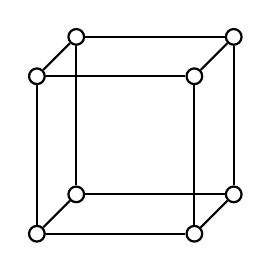
\begin{tikzpicture}
        [nodedecorate/.style={shape=circle,inner sep=2pt,draw,thick},%
          linedecorate/.style={-,thick}]
        %% nodes or vertices
        \foreach \nodename/\x/\y in {1/0/0, 2/2/0, 3/2/2, 4/0/2, 5/0.5/0.5,
          6/2.5/0.5, 7/2.5/2.5, 8/0.5/2.5}
        {
          \node (\nodename) at (\x,\y) [nodedecorate] {};
        }
        %% edges or lines
        \path
        \foreach \startnode/\endnode in {1/2, 2/3, 3/4, 4/1, 5/6, 6/7, 7/8,
          8/5, 1/5, 2/6, 3/7, 4/8}
        {
          (\startnode) edge[linedecorate] node {} (\endnode)
        };
        \end{tikzpicture}

        \caption{The $3$-hypercube graph}
        \label{fig:hypercube}
    \end{figure}
    
    Speaking generally, the symmetries of an object correspond with a group
    action that preserves the structure of the object.  The structure of a graph
    is determined entirely by its edges.
    \begin{definition}
        A \emph{graph automorphism} is a permutation of the vertices of a graph
        that preserves the edges.  That is, a permutation $\sigma: V \to V$ is a
        graph automorphism if for every $(u, v) \in E$, we have $(\sigma(u),
        \sigma(v)) \in E$.
        The \emph{automorphism group} of a graph is the set of all
        automorphisms of a graph with the group operation being composition of
        permutations.
    \end{definition}

    \begin{definition}
        The \emph{hyperoctahedral group} $H_n$ is the automorphism group of the
        $n$-hypercube.
    \end{definition}

    The wreath product is a construction on two permutation groups.
    Essentially, one permutation group shuffles copies of another permutation
    group.  In our example, $S_n$ permutes the binary variables, each of which
    has two states.  The copies of $S_2$ are each attached to one of the
    variables, and flip the values $0$ and $1$.  These copies of $S_2$ are then
    shuffled by the action of $S_n$.  We present a formal definition of the
    wreath product.
    \begin{definition}[\citet{Cam99}]
        Let $H$ and $K$ be permutation groups on the sets $\Gamma$ and $\Delta$
        respectively.  Let $\Omega = \Gamma \times \Delta$.  Think of $\Omega$
        as a fiber bundle over the set $\Delta$, with projection map $(\gamma,
        \delta) \mapsto \delta$; each fiber \mbox{$\Gamma_\delta = \{(\gamma, \delta)
        \mid \gamma \in \Gamma\}$} for fixed $\delta \in \Delta$ is isomorphic to
        $\Gamma$.  Let $B$ be the cartesian product of $|\Delta|$ copies of $H$,
        one acting on each fiber as $H$ acts on $\Gamma$.  Thus $B$ is the set
        of functions from $\Delta$ to $H$ with pointwise operations; the action
        on $\Gamma \times \Delta$ is given by
        \[
            f\cdot(\gamma, \delta) = (f(\delta) \cdot \gamma, \delta)
        \]
        where ($\cdot$) is used to denote group actions.  Let $T$ be a copy of
        the group $K$ permuting the fibers:
        \[
            k \cdot (\gamma, \delta) = (\gamma, k \cdot \delta).
        \]
        Then wreath product $H \wr K$ is defined to be the semidirect product $B
        \rtimes T$.
    \end{definition}

    The hypercube graph is has a number of nice properties.  In particular, it
    is distance-transitive; this allows us to characterize some of its
    irreducible representations easily.
    \begin{definition}
        A \emph{distance-transitive} graph is a graph such that given any two
        vertices $u_1$ and $v_1$ at distance $d$ and any other two vertices
        $u_2$ and $v_2$ also at distance $d$, there exists some automorphism
        $\sigma$ of the graph with $\sigma(u_1) = u_2$ and $\sigma(v_1) = v_2$.
    \end{definition}

    Let $(V, E)$ be a graph with automorphism group $G$.  Let \mbox{$U = \{ f : V \to
    \C\}$} be the vector space of complex-valued functions on the vertices of the
    graph.  The group $G$ has a permutation representation on $U$ defined for $f
    \in U$ and $x \in V$ as
    \begin{gather*}
        \sigma(f)(x) = f(\inv\sigma(x))
    \intertext{or, equivalently defined on delta functions as}
        \sigma(\delta_x) = \delta_{\sigma(x)}.
    \end{gather*}
    The permutation representation of the automorphism group of a
    distance-transitive graph decomposes into the eigenspaces of a particular
    matrix.  The information characterizing a graph may be encoded in an
    adjacency matrix.  The adjacency matrix of the $2$-hypercube is show below.
    \[
        \raisebox{-2.75em}{
        \begin{tikzpicture}
          \node (00) at (-1, 1) {00};
          \node (01) at (1, 1) {01};
          \node (10) at (-1, -1) {10};
          \node (11) at (1, -1) {11};
          \foreach \from/\to in {00/01, 01/11, 11/10, 10/00}
            \draw (\from) -- (\to);
        \end{tikzpicture}
        }
        \quad\text{has adjacency matrix}\qquad
        \kbordermatrix{
               & 00 & 01 & 10 & 11 \\
            00 &  0 &  1 &  1 &  0 \\
            01 &  1 &  0 &  0 &  1 \\
            10 &  1 &  0 &  0 &  1 \\
            11 &  0 &  1 &  1 &  0 \\
        }
    \]
    Of course, the adjacency matrix of a graph may be viewed as a linear
    transformation on $U$.

    The following theorem makes precise the relationship between the
    decomposition of $U$ into irreducible representations with the eigenspaces
    of the adjacency matrix of the graph.
    \begin{theorem}[\citet{Sta84}]
        Let $G$ be the automorphism group of a distance-transitive graph.  Let
        $U$ be the permutation representation of $G$ on the complex-valued
        functions on the vertices of the graph.  Then $U$ decomposes as
        \[
            U = U_{\lambda_1} \oplus \cdots \oplus U_{\lambda_k}
        \]
        where the $\lambda_i$ are distinct eigenvalues of the adjacency matrix,
        $U_{\lambda_i}$ is the eigenspace corresponding to $\lambda_i$, and the
        $U_{\lambda_i}$ are also distinct irreducible representations of $G$.
    \end{theorem}

    The adjacency matrices and eigenspaces for the $n$-hypercubes have a
    recursive structure.
    \begin{theorem}[\cite{CW06}]
        The adjacency matrix $Q_n$ for the $n$-hypercube, with vertices ordered
        lexicographically, is given by the following recursively defined block
        matrix
        \[
            Q_0 = \begin{bmatrix} \;0\; \end{bmatrix}
            \qquad
            \text{and}
            \qquad
            Q_n = \begin{bmatrix}
                Q_{n-1} & I \\
                I & Q_{n-1}
            \end{bmatrix}
            \qquad
            \text{for $n \ge 1$}
        \]
        where $I$ is the $2^{n-1}\times 2^{n-1}$ identity matrix.
    \end{theorem}

    \begin{theorem}[\cite{CW06}]
        If $v$ is an eigenvector of $Q_{n-1}$ with eigenvalue $\lambda$ then the
        concatenated vectors $\adel{v_1, \ldots, v_{2^{n-1}},v_1, \ldots,
        v_{2^{n-1}}}$ and $\adel{v_1, \ldots, v_{2^{n-1}}, -v_1, \ldots,
        -v_{2^{n-1}}}$ are eigenvectors of $Q_n$ with eigenvalues $\lambda +1$
        and $\lambda - 1$ respectively.
    \end{theorem}

    \begin{theorem}[\cite{CW06}]
        The eigenvectors of $Q_n$ are the Walsh functions of dimension $2^n$.
        The eigenvalues are given by $\lambda_k = 2k - n$ for $k \in \{0,
        \ldots, n\}$, and have multiplicity $\binom{n}{k}$.
    \end{theorem}

    These theorems give us a full characterization of the permutation
    representation of the hyperoctahedral group.

    The above decomposition of the permutation representation of the
    hyperoctahedral group on $\{0, 1\}^n$ gives us a way to enumerate the $S_2
    \wr S_n$ invariant log-linear models.

    We label the irreducible representations in $\R^{2^n}$ be their eigenvalues,
    which take on the $n+1$ values $-n, -n + 2, \ldots, n - 2, n$.  The
    $U_n$ eigenspace with eigenvalue $\lambda = n$ contains the all-ones vector $(1,1,
    \ldots, 1)$.  Every other eigenspace is perpendicular to $U_n$, and thus
    contains vectors that sum to zero.  This means that every invariant
    log-linear model must contain the irreducible representation $U_n$.  Every
    invariant space is the direct product of some of the $U_\lambda$.  Excluding
    $U_n$, there are $n$ irreducible representations, and thus $2^n$ possible
    invariant models.

    (Define hierarchical log-linear models.)

    The hierarchical log-linear model with all size $k$ facets corresponds with
    the representation $U_n \oplus U_{n-2} \oplus U_{n-2\cdot2}\cdots \oplus U_{2k}$.
    We can verify this with the computation
    \[
        \ldots
    \]

\section{k-Subsets}

    Let $n$ and $k$ be positive integers.  Let the space of states $\xs$ be the
    collection of all subsets of size $k$ of $\{1, \ldots, n\}$.

    This space of states turns up in approval voting, where voters are asked to
    select their $k$ favorite candidates out of $n$ choices.



\appendix


% \nocitep{*}
\chapter{Orphaned Sections}

\section{Algebraic Statistics}

    Algebraic statistics is a relatively new field that examines statistical
    questions using algebraic geometry and commutative algebra.  Once a problem
    has been cast in the language of algebra, a number of computational tools
    can be brought to bear.  For example, one of the early papers in the field
    analyzed contingency tables using Monte Carlo sampling computed with Gröbner
    bases \citep{DS98}.

    Algebraic statistics also offers a geometric point of view on statistical
    models; the tendency is toward intrinsically defined objects in lieu of
    explicit coordinate systems.  In this light, algebraic statistics might be
    seen as in the tradition of information geometry, a field pioneered in the
    1980s that applied the techniques of Riemannian geometry to probability
    models (see for example \citep{Ama}).

    An introduction to the field of algebraic statistics may be found in the
    collection of lecture notes \citep{DSS08}.  Algebraic statistics has also
    been applied to computational biology \citep{ASCB}.


\section{Markov Random Fields}
    \label{sec:rbm-def}

    The Restricted Boltzmann Machine is an instance of a \emph{graphical model}.
    A graphical model is a probabilistic model for which a graph (directed or
    undirected) represents the conditional independence structure between random
    variables.  Several types of graphical models have become popular for
    applications in machine learning; Chapter 17 of \citep{EOSL} is an overview
    of undirected graphical models and additionally contains references to the
    large body of literature.  From the algebro-geometric point of view,
    graphical models in general are discussed in Chapter 3 of \citep{DSS08} and
    directed graphical models, known as \emph{Bayesian networks}, are discussed
    in \citep{GSS}.  In our exposition we only introduce undirected models.

    \begin{definition}
        We describe a \emph{Markov random field}, i.e. an undirected graphical
        model.  Let $G$ be an undirected graph with vertex set $V$.  Let
        $\{X_\alpha\}_{\alpha \in V}$ be random variables indexed by the
        vertices.  The joint probability of $(X_\alpha)_{\alpha \in V}$ is said
        to factor according to $G$ if for any pair of vertices $\beta, \gamma
        \in V$ that are not adjacent, the random variables $X_\beta, X_\gamma$
        are conditionally independent given the variables at the other vertices.
        That is,
        \[
            \text{$X$ and $Y$ not adjacent}
            \Longleftrightarrow
            X_\beta \perp X_\gamma \mid 
            \{X_\alpha; \text{for } \alpha \ne \beta, \alpha \ne \gamma\}.
        \]
        A Markov random field is any such collection of random variables that
        factor according to an undirected graph.
    \end{definition}

    Roughly speaking, the edges in the graph record which variables influence
    which other variables.  If the graph is relatively sparse, then there are
    strong restrictions on the interactions between variables.  For example, a
    totally disconnected graph indicates that the variables are all independent.
    In contrast, a complete graph places no restrictions at all on the
    variables' joint distribution.
    
    With the assumption that distributions are strictly positive, there is an
    equivalent characterization of a graphical model.

    \begin{theorem}[Hammersley-Clifford]
        The random variables $(X_\alpha)_\alpha$ indexed by the vertices of an
        undirected graph $G$ factor according to $G$ if and only if their
        joint probability density factors as
        \[
            p(x) = \prod_{S \in C(G)} f_S(x_S)
        \]
        where the $S$ are maximal complete subgraphs (cliques) of $G$, $x_S$ is
        the restriction of $x$ to $S$, and $f_S$ is a function on the variables in
        $S$.
    \end{theorem}

    The graphical models that we consider have a particularly simple structure;
    the variables have binary values and all interactions are pairwise.
    Following the machine learning literature, we refer to binary-valued random
    variables and their corresponding vertices as `units'.

\section{Sufficient Statistic}
    \begin{definition}
        A \emph{sufficient statistic} of a parametrized model is a linear
        function $T$ of the data $u : \xs \to \N$ such that the log-likelihood
        factors as
        \[
            l(\theta; u) = f(T(u), \theta) + g(u)
        \]
        that is, that in order to estimate the value of the parameter, we do not
        need the data, only the sufficient statistic.
    \end{definition}

    \begin{theorem}[Pitman-Koopman-Darmois]
        Exponential families are the `largest' possible with \ldots
    \end{theorem}

    The essential point is that
    \[
        l(p; z) = \log p(z_1) + \cdots + \log p(z_m) 
    \]
    so log-probabilities are additive with respect to counts of observations.
    If we want to summarize our data through a linear transformation of the
    counts, then we must work with log-probabilities.  Thus linear subspaces of
    the log-probabilities are a natural choice for models.


\backmatter

\bibliographystyle{hmcmath}
\bibliography{thesis}

\printindex


\end{document}
